\chapter{Project Context}

\section*{Introduction}

The aim of this chapter is to present the general framework of the Korpor project, a solution dedicated to real estate investment. In this chapter, we'll discuss successively:

The presentation of the host organization and the context and challenges of the real estate sector and the analysis of existing solutions and identification of their limitations.


\section{Project Context}

This work is part of the end-of-study project for the national diploma of Applied Bachelor's degree in Computer Science from the Higher Institute of Computer Science and Mathematics of Monastir (ISIMM) for the year 2024/2025. we has the opportunity to do our end-of-study internship at the company
<< KZ IT Services >>, under the supervision of Mr. Khalil Zouari.

\section{Hosting Company}

The purpose of this section is to present the company within which I developed my project, as shown in Figure \ref{fig:hosting-company}.

\begin{figure}[htbp]
    \centering
    
\includegraphics[width=0.2\textwidth]{images/company-logo.png}
    \caption{Hosting Company << KZ IT Services >>}
    \label{fig:hosting-company}
\end{figure}

\newpage
\begin{table}[htbp]
    \centering
    \caption{KZ IT Services - Company Information}
    \label{tab:kz_it_services_info}
    \renewcommand{\arraystretch}{1.3}
    \begin{tabular}{|l|p{0.7\textwidth}|}
        \hline
        \rowcolor{primary!10}
        \textbf{Aspect} & \textbf{Details} \\
        \hline
        Company Name & KZ IT Services \\
        \hline
        \rowcolor{background!50}
        Specialization & Custom software development, IT solutions, Digital transformation \\
        \hline
        Mission Focus & Delivering innovative, robust, and scalable IT solutions to drive client efficiency and success through quality and continuous improvement. \\
        \hline
        \rowcolor{background!50}
        Size & 2-10 employees \\
        \hline
        \rowcolor{background!50}
        Location & Djerba, Tunisia \\
        \hline
    \end{tabular}
\end{table}

\textbf{\textcolor{primary}{KZ IT Services}} is a dynamic software company dedicated to delivering innovative IT solutions tailored to modern business needs. they are specialize in designing and developing robust, scalable applications that drive efficiency and digital transformation. thier experienced team leverages cutting-edge technology to create customized software that exceeds client expectations. With a strong commitment to quality and continuous improvement, they build lasting partnerships based on trust and excellence. At << KZ IT Services >>, innovation is at the core of everything they do, empowering thier clients to achieve sustainable growth and success.

\section{Preliminary Study}

This preliminary study provides a review of some existing investment and asset management platforms. Further, the next section identifies some key concepts that will lead to further understanding of the domain in question.

\subsection{Existing Solutions Study}

After conducting extensive research on investment platforms similar to our concept across the global market, we carefully analyzed numerous applications based on their performance metrics and market position. From this comprehensive study, we specifically selected << Aseel >> \cite{AssilEyeInstitute} and << Stake >> \cite{StakeWebsite} for in-depth analysis \cite{G2CompetitiveAnalysis2024, AsanaCompetitiveAnalysis2024} due to their exceptional performance and status as leading companies in the real estate investment platform sector.

\subsubsection{The Aseel Platform}

\textbf{\textcolor{primary}{Aseel}} \cite{AssilEyeInstitute} is a portal through which users can invest in different real estate projects with ease. The interface allows the clients to surf various investment opportunities, view 

\newpage

the details of the properties, and then make an informed decision. Aseel introduces transparency in the investment process by offering financial data, updates regarding projects, and returns that are estimated. This platform comes with an easy-to-use dashboard through which one tracks their investments and manages their assets without any hassle. The interface of the Aseel Platform is shown in Figure \ref{fig:aseel-platform}.


\begin{figure}[htbp]
    \centering
    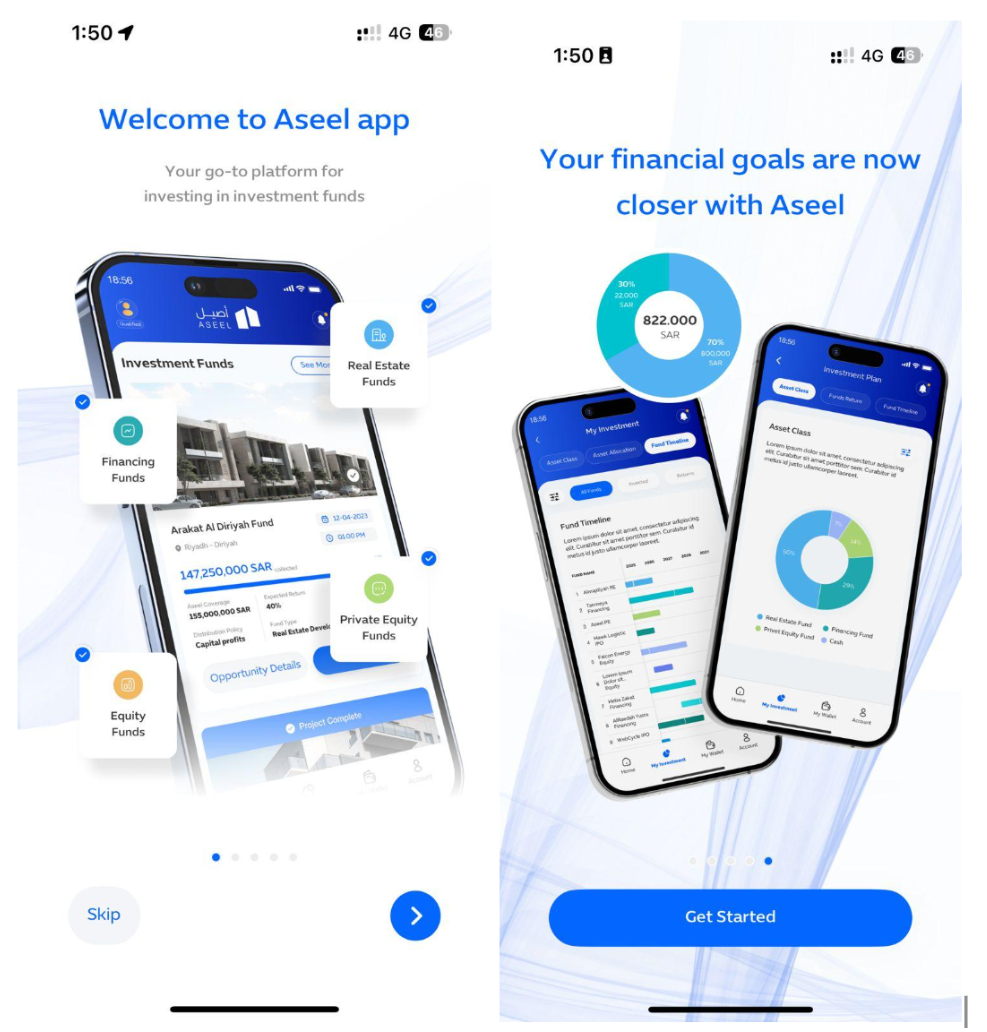
\includegraphics[width=0.65\textwidth]{images/Interface-of-the Aseel Platform.png}
    \caption{Interface of << The Aseel Platform >>}
    \label{fig:aseel-platform}
\end{figure}

% \begin{center}
%     \vspace{0.5em}
%     \begin{tikzpicture}
%         \draw[primary, line width=1pt] (0,0) -- (0.3\textwidth,0);
%         \draw[accent, line width=0.7pt] (0.1\textwidth,-0.07) -- (0.4\textwidth,0.07);
%         \fill[primary] (0,0) circle (2pt);
%         \fill[accent] (0.3\textwidth,0) circle (2pt);
%     \end{tikzpicture}
%     \vspace{0.5em}
% \end{center}

\subsubsection{The Stake Platform}

\textbf{\textcolor{primary}{Stake}} \cite{StakeWebsite} is an online investment platform that deals with real estate crowdfunding. It provides the opportunity to invest in fractions of property ownership, hence diversifying a portfolio without huge capital. On Stake, there are AI-powered recommendations based on user preferences, seamless payment integration, and a secure environment for investment. Besides, liquidity is guaranteed by enabling exit options for investors who may want to sell their shares in ongoing projects. Figure \ref{fig:stake-platform} illustrates the interface of the Stake Platform.

\newpage
\thispagestyle{empty}
\newpage

\begin{figure}[htbp]
    \centering
    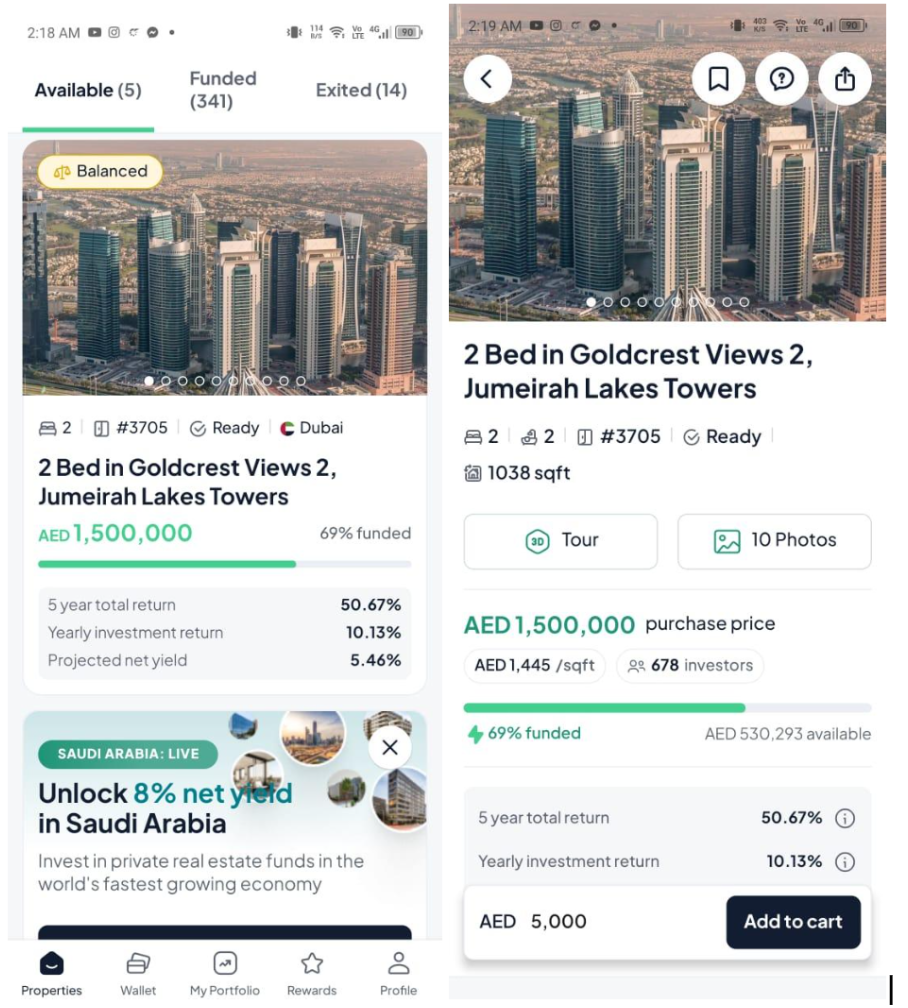
\includegraphics[width=0.65\textwidth]{images/Interface-of-the Stake Platform.png}
    \caption{Interface of << The Stake Platform >>}
    \label{fig:stake-platform}
\end{figure}

\subsection{Comparative and Critical Analysis}

We can summarize all that comes from our analysis based on a number of criteria used for the evaluation of these applications \cite{LyssnaUXAnalysis2024, StrategicManagementInsightCA2024}.

\begin{itemize}
    \item \textbf{Speed (C1)}: The platform should obtain value for the user as fast as possible and effectively, anticipating their proliferating expectations.
    \item \textbf{Costs (C2)}: With minimum software development costs, it is important to keep the pricing predictable and acceptable.
    \item \textbf{Quality (C3)}: Since the market expects quality, any kind of error might affect brand reputation. Improvement of the platform should be regular.
    \item \textbf{Reliability (C4)}: Since modern-day investment platforms need to make sure of minimum downtime and maximum availability of services, this factor is critical.
    \item \textbf{Security (C5)}: Such an investment platform enforces access rights, roles, and contribution rights through a powerful security system.
    \item \textbf{Performance (C6)}: Crucial features include AI-powered recommendations going through seamlessly, easy transaction tracking, and investment monitoring.
    \item \textbf{Stability (C7)}: The platform should have a proven track record, regular updates, and a large user base to ensure its longevity.
    \item \textbf{Resilience (C8)}: In order to prevent data loss and guarantee a smooth experience for investors, it must be able to restore lost functionalities should issues occur.
    \item \textbf{User Experience (C9)}: The interface should be intuitive and user-friendly, hence allowing investors to move with ease through it, thus making wiser decisions.
\end{itemize}

Table \ref{tab:evaluation} presents the evaluation of the existing solutions based on these criteria:

\begin{table}[htbp]
    \centering
    \caption{Evaluation Table}
    \label{tab:evaluation}
    \renewcommand{\arraystretch}{1.3}
    \begin{tabular}{|>{\columncolor{background}}c|*{9}{>{\centering\arraybackslash}p{0.7cm}|}}
        \hline
        \rowcolor{primary!15}
        \textcolor{primary}{\textbf{Solution}} & 
        \textcolor{primary}{\textbf{C1}} & 
        \textcolor{primary}{\textbf{C2}} & 
        \textcolor{primary}{\textbf{C3}} & 
        \textcolor{primary}{\textbf{C4}} & 
        \textcolor{primary}{\textbf{C5}} & 
        \textcolor{primary}{\textbf{C6}} & 
        \textcolor{primary}{\textbf{C7}} & 
        \textcolor{primary}{\textbf{C8}} & 
        \textcolor{primary}{\textbf{C9}} \\
        \hline
        \textbf{Stake} & \textcolor{primary}{\checkmark} & \textcolor{primary}{\checkmark} & \textcolor{primary}{\checkmark} & \textcolor{primary}{\checkmark} & \textcolor{primary}{\checkmark} & $\times$ & \textcolor{primary}{\checkmark} & \textcolor{primary}{\checkmark} & \textcolor{primary}{\checkmark} \\
        \hline
        \rowcolor{background!50}
        \textbf{Aseel} & \textcolor{primary}{\checkmark} & \textcolor{primary}{\checkmark} & \textcolor{primary}{\checkmark} & $\times$ & \textcolor{primary}{\checkmark} & $\times$ & \textcolor{primary}{\checkmark} & $\times$ & \textcolor{primary}{\checkmark} \\
        \hline
    \end{tabular}
\end{table}

\subsection{Proposed Solution}

The \textbf{\textcolor{primary}{Korpor}} platform is a dual-benefit real estate solution for agencies and investors, prioritizing a symbiotic ecosystem where agency efficiency enhances investor opportunities and experience.

\subsubsection*{Benefits for Real Estate Agencies}
\begin{itemize}
    \item \textbf{Expanded Market Reach \& Sales Scalability:} Showcase properties to more investors and scale sales via blockchain-recorded fractional ownership, broadening the investor base.
    \item \textbf{Streamlined Operations \& Enhanced Presence:} Efficiently manage listings, client interactions, and bolster digital brand image, gaining insights into market trends.
\end{itemize}

\subsubsection*{Benefits for Investors}
\begin{itemize}
    \item \textbf{Accessible \& Simplified Investments:} Discover diverse real estate opportunities, including fractional ownership, with simplified processes that handle paperwork and rent collection.
    \item \textbf{AI-Powered Guidance \& Secure Transactions:} Receive personalized AI recommendations and experience secure, transparent, blockchain-recorded transactions with robust regulatory adherence.
    \item \textbf{Seamless Portfolio Management:} Track investments in real-time via a user-friendly dashboard and mobile app.
\end{itemize}


\section{Development methodology}

Meeting project delivery deadlines is a critical challenge in software development. Common issues include insufficient technical specifications, poor time management with emerging technologies, and sudden requirement changes. To address these challenges, we follow an agile methodology using Git \cite{GitWebsite} for version control and GitHub \cite{GithubWebsite} for collaborative development.

\subsection{SCRUM}

\textbf{\textcolor{primary}{Scrum}} is an agile development approach that is used to create software using incremental and iterative methods. Scrum is a quick, flexible, and efficient agile methodology that is intended to provide value to the client at every stage of the project's development \cite{ScrumGuide2020}. Scrum is founded on empiricism and lean thinking, employing an iterative, incremental approach guided by the three pillars of transparency, inspection, and adaptation \cite{AtlassianScrumPillars, ScrumGuide2020}. Scrum's main goal is to meet customer needs by fostering an atmosphere of open communication, group accountability, and constant improvement, underpinned by the Scrum values of Commitment, Focus, Openness, Respect, and Courage \cite{ScrumGuide2020}. The development process begins with a broad concept of what must be constructed, developing a list of features that the product owner desires, and arranging them according to priority (product backlog).

\begin{figure}[ht!]
    \centering
    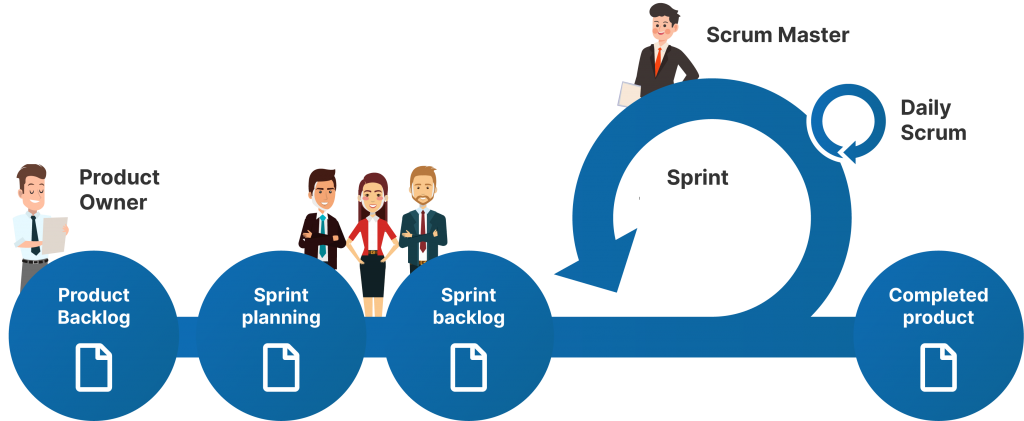
\includegraphics[width=0.9\textwidth]{images/agile.png}
    \caption{Agile Scrum Framework Process}
    \label{fig:agile-scrum}
\end{figure}

\subsection{Agile Scrum roles and responsibilities}

\subsubsection{The Product Owner}

The Product Owner understands the customer and business requirements, then creates and manages the product backlog based on those requirements. Their key responsibilities include managing the scrum backlog, overseeing release management, and handling stakeholder management to ensure project alignment with business objectives.

\subsubsection{Developers}

In Scrum, the term developer or team member refers to anyone who plays a role in the development and support of the product and can include researchers, architects, designers, programmers, etc. Developers are responsible for delivering the work through the sprint and ensuring transparency during the sprint by meeting daily at the daily scrum to discuss progress and challenges.

\subsubsection{Scrum Master}

The Scrum Master is the role responsible for gluing everything together and ensuring that scrum is being done well. In practical terms, that means they help the product owner define value, the development team deliver the value, and the scrum team get better. The Scrum Master focuses on maintaining transparency, promoting empiricism, encouraging self-organization, and facilitating the Scrum events effectively.

\subsection{The Scrum Events}

The Scrum events are key elements of the Scrum Framework. They provide regular opportunities for enacting the Scrum pillars of Inspection, Adaptation and Transparency \cite{ScrumGuide2020}. In addition, they help teams keep aligned with the Sprint and Product Goals, improve Developer productivity, and remove impediments and reduce the need to schedule too many additional meetings.

\begin{itemize}
    \item \textbf{Sprint}: All work in Scrum is done in a series of short projects called Sprints. This enables rapid feedback loops.
    
    \item \textbf{Sprint Planning}: The Sprint starts with a planning session in which the Developers plan the work they intend to do in the Sprint. This plan creates a shared understanding and alignment among the team.
    
    \item \textbf{Daily Scrum}: The Developers meet daily to inspect their progress toward the Sprint Goal, discuss any challenges they've run into, and tweak their plan for the next day as needed.
    
    \item \textbf{Sprint Review}: At the end of the Sprint, the Scrum Team meets with stakeholders to show what they have accomplished and get feedback.
    
    \item \textbf{Sprint Retrospective}: Finally, the Scrum Team gets together to discuss how the Sprint went and if there are things they could do differently and improve in the next Sprint.
\end{itemize}

\section*{Conclusion}

It is clear that planning and methodology are essential pillars to ensure the success of the project. By fully understanding the project framework, including the host organization's expectations and the challenges ahead, the team is better prepared to meet the challenges ahead.

This chapter lays the solid foundation on which the entire project will be built, providing a valuable guide for the next steps. The next chapter will allow us to analyze and specify the requirements developed for our project. 